% !TEX TS-program = xelatex
% !TEX encoding = UTF-8 Unicode
% !Mode:: "TeX:UTF-8"

\documentclass{resume}
\usepackage{
  zh_CN-Adobefonts_external
} % Simplified Chinese Support using external fonts (./fonts/zh_CN-Adobe/)
% \usepackage{NotoSansSC_external}
% \usepackage{NotoSerifCJKsc_external}
% \usepackage{zh_CN-Adobefonts_internal} % Simplified Chinese Support using system fonts
\usepackage{linespacing_fix} % disable extra space before next section
\usepackage{cite}
\usepackage{graphicx}
\usepackage{tabu}
\usepackage{multirow}
\usepackage{progressbar}
\begin{document}
\pagenumbering{gobble} % suppress displaying page number
\begin{center}
  \Large{ \begin{tabu}{ c l r } \multirow{4}{1in}{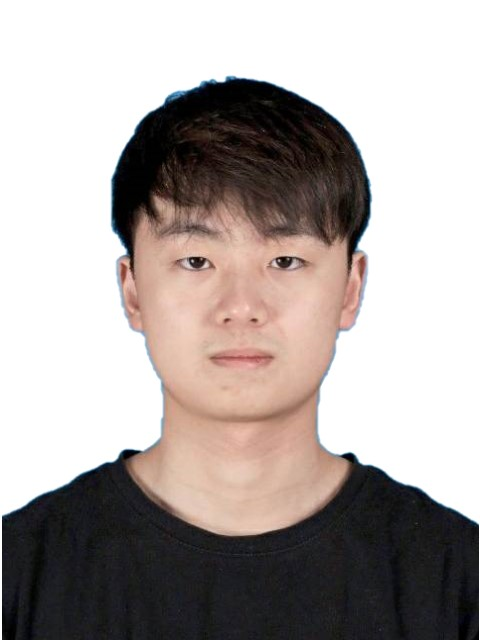
\includegraphics[width=0.78in]{author.jpg}} & \textbf{周志宇} \\ & \email{zhouzhiyuwhu@gmail.com} \\ & \phone{(+86) 187-620-29645} \\ & \github[github.com/zzywhu]{https://github.com/zzywhu}\end{tabu} }
\end{center}

\section{\faGraduationCap\  教育背景}
\datedsubsection{\textbf{武汉大学}, 武汉, 湖北}{2024 -- 至今} \textit{在读博士研究生（直博）}\ 遥感科学与技术,
预计 2029 年 6 月毕业 \datedsubsection{\textbf{武汉大学}, 武汉, 湖北}{2020 -- 2024}
\textit{学士}\ 摄影测量与遥感

\section{\faUsers\ 实习/项目经历}
% \datedsubsection{\textbf{中船重工716研究所}，连云港，江苏}{2024年6 -- 2024年9月}
% \role{高新技术部SLAM算法工程师}{实习}

% 作为主要成员参与无人船高精度多传感器空间标定算法设计，完成包括激光雷达、毫米波雷达、可见光相机与红外相机等传感器的子像素级标定项目开发。

% \begin{itemize}
%   \item 设计了激光雷达-相机的通用外参立体标志块及Linux/Win平台下全自动数据采集与标定算法。
%   \item 实现标定数据ros数据包的自动解码与标定文件的自动排列。
%   \item 基于c++/ros/pcl/ceres/opencv开发了基于立体标定块的多模态特征提取与关联算法，实现子像素级外参标定(精度小于一个像素),算法现长期运行于连岛无人船实验基地。
% \end{itemize}

\datedsubsection{\textbf{智元机器人}，上海数采中心}{2025 年6月 -- 9月}
\role{SLAM算法工程师}{实习}
参与轮式机器人底盘多传感器 SLAM 系统维护，并负责基于反光条的高精度回充定位算法开发。

\datedsubsection{\textbf{中国长江三峡集团}，白鹤滩，四川}{2024年11月 -- 2025年4月}
\role{多传感器融合定位建图算法设计}{合作项目}
面向水电站长距离、弯曲隧道等退化环境，开发基于激光雷达反射率与惯性单元紧耦合的鲁棒定位建图算法。

\datedsubsection{\textbf{中观自动化}，武汉，湖北}{2024年9月 -- 2025年2月}
\role{机械式主动旋转激光雷达手持扫描仪（RigelSLAM）开发}{合作项目}
负责电机-激光雷达空间标定、在线优化及点云地图精细化算法开发。

% Reference Test
%\datedsubsection{\textbf{Paper Title\cite{zaharia2012resilient}}}{May. 2015}
%An xxx optimized for xxx\cite{verma2015large}
%\begin{itemize}
%  \item main contribution
%\end{itemize}

\section{\faInfo\ 论文\&专利}
% increase linespacing [parsep=0.5ex]
\begin{itemize}[parsep=0.5ex]
  \item \textbf{Z. Zhou}, Z. Gao, and J. Xu, ``Tracking by Detection: Robust Indoor RGB-D Odometry Leveraging Key Local Manhattan World,'' IEEE Robotics and Automation Letters, 2024.

  \item \textbf{Z. Zhou}, Z. Gao, Y. Li, and H. Zhen, ``EasyColor: Reflectivity Assisted Dense Point Cloud RGB Colorizing Without Accurate Time Synchronization and Extrinsic Calibration,'' IEEE Robotics and Automation Letters, 2026.

  \item \textbf{Z. Zhou} and Z. Gao, ``EasyCalib: A Novel Target for High-Accuracy Fully-Automatic Extrinsic Calibration of Camera and LiDAR,'' IEEE Transactions on Instrumentation and Measurement, 2026.

  \item \textbf{Z. Zhou}, B. Guan, W. Yang, Z. Gao, and H. Fang, ``Hi-Nav: Hierarchical Framework for Continuous Vision-Language Navigation via Map Guidance and Waypoint Reasoning,'' European Conference on Computer Vision, 2026.

  \item \textbf{Z. Zhou} and Z. Gao, ``R3LIO: Robust Reflectivity-Assisted Rotating LiDAR-Inertial Odometry for Degenerate and Unstructured Environments,'' ISPRS Journal of Photogrammetry and Remote Sensing, 2026.

  \item 高智，\textbf{周志宇}等，室外大场景激光雷达点云地图的生成方法及装置，国家发明专利（学生一作，已授权）

  \item 高智，\textbf{周志宇}等，基于激光雷达与电机的扩展关系模型的点云地图生成方法，国家发明专利（学生一作，已授权）

  \item 高智，\textbf{周志宇}等，一种针对弱结构长隧道环境的激光惯性里程计算法，国家发明专利（学生一作，已授权）
\end{itemize}

\section{\faHeartO\ 获奖情况}
\datedline{\textit{全国特等奖（3/10）}, 第十八届“挑战杯”全国大学生课外学术科研作品竞赛}{2023 年12 月}
\datedline{ \textit{个人奖项}，武汉大学优秀本科毕业生}{2024 年6 月} \datedline{ \textit{个人奖项}，武汉大学优秀本科毕业论文}{2024 年6 月}
\datedline{ \textit{个人奖学金}，武汉大学知卓奖学金}{2024 年9 月} \datedline{ \textit{个人奖学金}，武汉大学研究生出国（境）交流资助项目奖学金}{2024 年10 月}

\section{\faCogs\ 专业技能}
\begin{itemize}[parsep=0.5ex]
  \item 编程语言：C++、Python、Matlab

  \item 平台：Linux、ROS
\end{itemize}

%% Reference
%\newpage
%\bibliographystyle{IEEETran}
%\bibliography{mycite}
\end{document}